\section{Einführung und institutionelle Grundlagen}

\textbf{Elemente des Jahresabschlusses}: 
\begin{itemize}
	\item \textbf{Bilanz}, Gewinn- und Verlustrechnung (\textbf{GuV})
	\item nur bei Kapitalgesellschaft: \textbf{Anhang} für GuV und \textbf{Lagerbericht}
	\item Weitere Publizitätspflichten für börsennotierte Unternehmen:
	\begin{itemize}
		\item Zwischenberichte in Form verkürzter Jahresabschlüsse
		\item Ad-Hoc-Publizität: Unverzügliches publizieren von Insiderinformationen
		\item Beteiligungsverhältnisse
	\end{itemize}
	\item Ergebnis des externen Rechnungswesens: \textbf{Einzelabschlusses} oder \textbf{Konzernabschlusses}
	\item Pflicht zur Erstellung für alle Kaufleute
\end{itemize}
\bigskip
\textbf{Grundaufbau und Inhalt der Bilanz}:
\begin{itemize}
	\item Aufbau s.S18
	\item Hauptfunktionen des externen Rechnungswesens: 
	\begin{itemize}
		\item Bereitstellung von \textbf{entscheidungsnützlicher Informationen} (z.B. Kreditvergabe, Kauf/Verkauf von Anteilen, Handelsbeziehungen) $\rightarrow$ Entscheidungsfunktion, Prognosefähigkeit, Verlässlichkeit für Adressaten
		\item \textbf{Anspruchsbemessung und Vertragsgestaltung} (z.B. Zahlungsansprüche) $\rightarrow$ Verhaltenssteuerungsfunktion, Rechenschaftslegung, Verlässlichkeit für Adressaten
		\item Adressaten unternehmensintern (z.B. Eigentümer, Management) oder -extern (z.B. Gläubiger, Investoren)
	\end{itemize} 
\end{itemize}
\bigskip
\textbf{Charakteristika der externen Rechnungslegung}:
\begin{itemize}
	\item Objektivierung (möglichst objektive Bewertung)
	\item Periodisierung (Ermittlung des Periodengewinns)
	\item Asymmetrische Erfassung von Gewinnen und Verlusten (Vorsichtsprinzip)
	\item Betonung finanzieller Größen (Aggregierbarkeit durch Bilanzierung und Bewertung)
	\item Standardisierung (Regeln und Standards für Vergleichbarkeit)
\end{itemize}
\bigskip
\textbf{Institutioneller Rahmen der Rechnungslegung}:
Aufgrund der Trennung von Ersteller und Benutzern der Unternehmensrechnung können Friktionen entstehen. \\
$\rightarrow$ Institutioneller Rahmen zur Sicherstellung der Qualität der externen Rechnungslegung, z.B.
\begin{itemize}
	\item gesetzliche Regelungen
	\item Abschlussprüfungen
	\item \textbf{Corporate Governance}-Regeln: Rechtlicher und faktischer Ordnungsrahmen für die
	Leitung und Überwachung eines Unternehmens
\end{itemize}
\begin{center}
	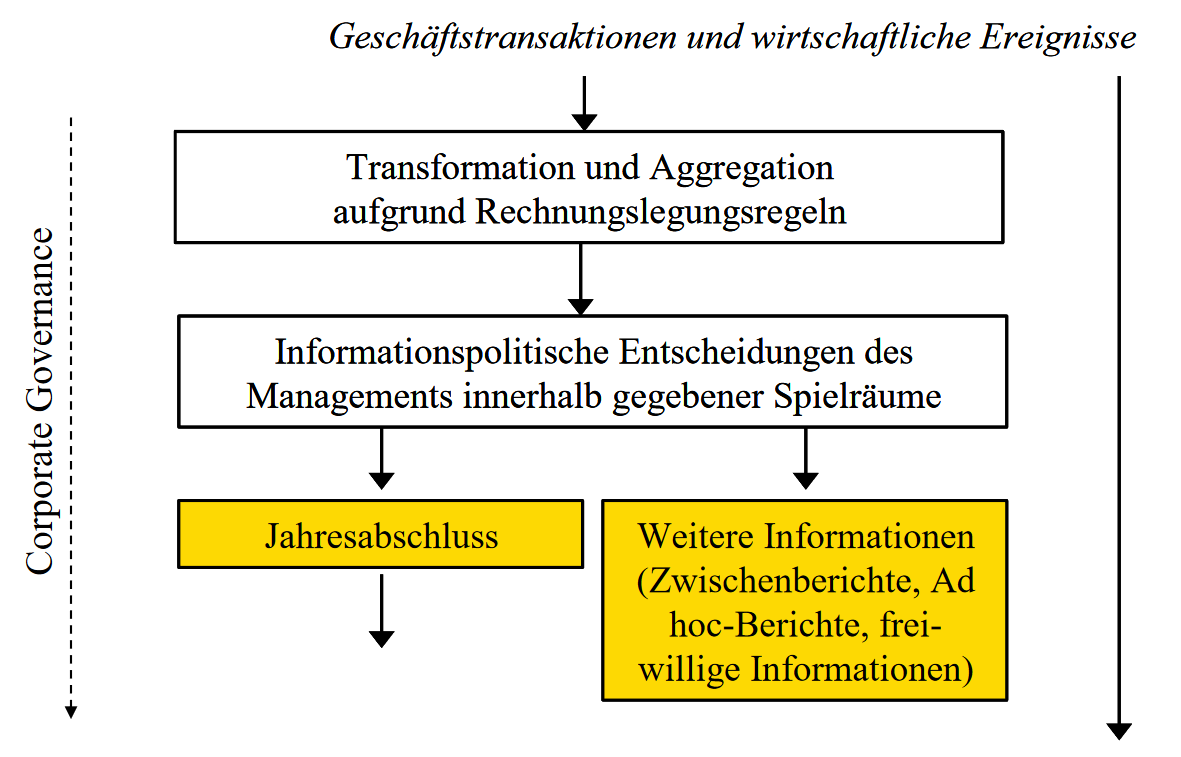
\includegraphics[width=0.7\textwidth]{images/ir1.png}
	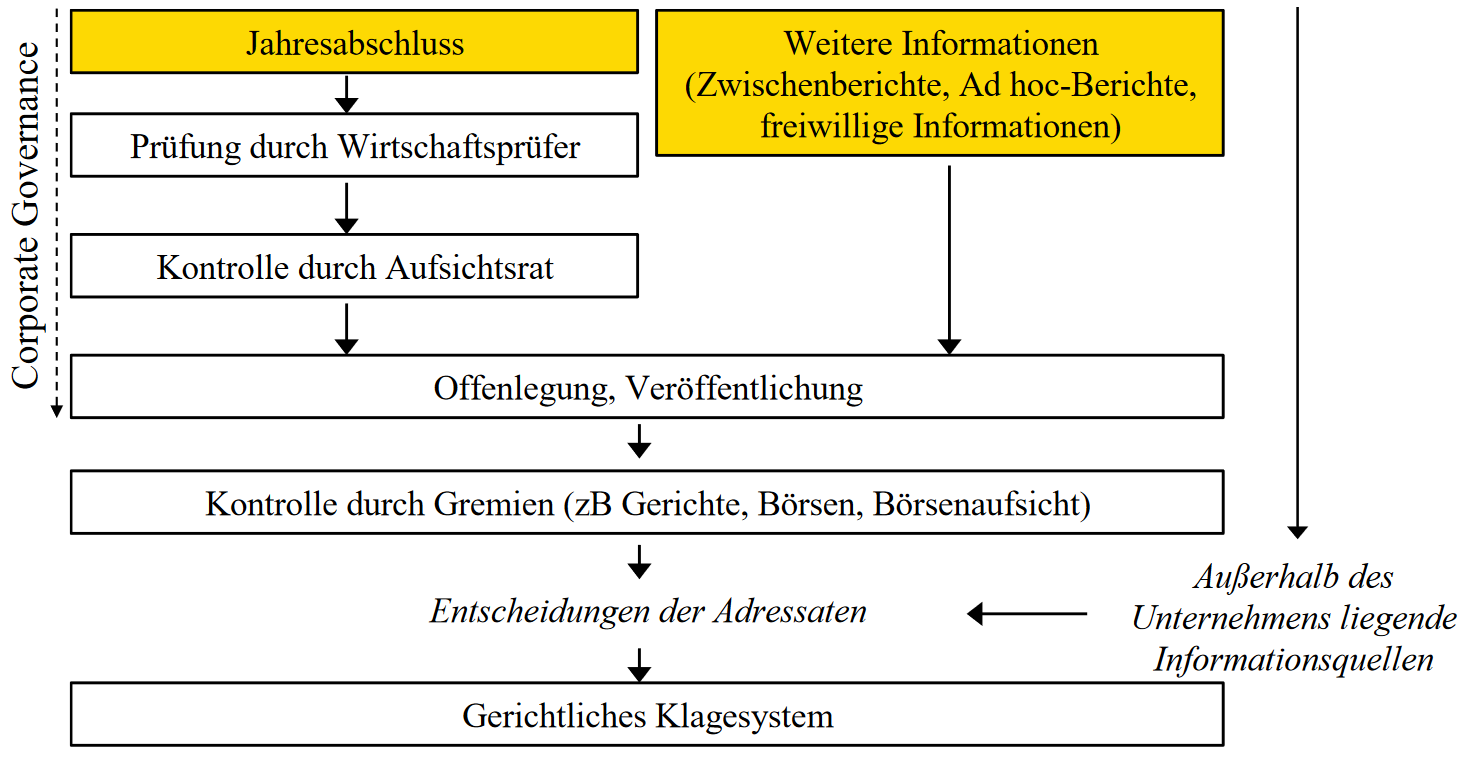
\includegraphics[width=0.8\textwidth]{images/ir2.png}
\end{center}

\textbf{Regulierung der Rechnungslegung}: 
\begin{itemize}
	\item \textbf{Ziele}: Schutz schwacher Adressatengruppen, Begrenzung externer Effekte
	\item Quellen der Regulierung: Gesetzliche Quellen, Standardsetter (z.B. Gremien), Empfehlungen (z.B. von Verbänden/Experten)
	\item Weiterentwicklung der Rechnungslegung zielt auf eine stärkere Kapitalmarktorientierung
\end{itemize}